%%%%%%%%%%%%%%%%%%%%%%%%%%%%%%%%%%%%%%%%%
% Simple Sectioned Essay Template
% LaTeX Template
%
% This template has been downloaded from:
% http://www.latextemplates.com
%
% Note:
% The \lipsum[#] commands throughout this template generate dummy text
% to fill the template out. These commands should all be removed when 
% writing essay content.
%
%%%%%%%%%%%%%%%%%%%%%%%%%%%%%%%%%%%%%%%%%

%----------------------------------------------------------------------------------------
%	PACKAGES AND OTHER DOCUMENT CONFIGURATIONS
%----------------------------------------------------------------------------------------

\documentclass[12pt]{article} % Default font size is 12pt, it can be changed here

\usepackage{geometry} % Required to change the page size to A4
\geometry{a4paper} % Set the page size to be A4 as opposed to the default US Letter

\usepackage{graphicx} % Required for including pictures

\usepackage{float} % Allows putting an [H] in \begin{figure} to specify the exact location of the figure
\usepackage{wrapfig} % Allows in-line images such as the example fish picture

\usepackage{url} % Allows for urls to be formatted decently well

\usepackage{natbib}

% \usepackage{lipsum} % Used for inserting dummy 'Lorem ipsum' text into the template

\linespread{1.2} % Line spacing

%\setlength\parindent{0pt} % Uncomment to remove all indentation from paragraphs

\graphicspath{{img/}} % Specifies the directory where pictures are stored

\begin{document}

%----------------------------------------------------------------------------------------
%	TITLE PAGE
%----------------------------------------------------------------------------------------

\begin{titlepage}

\newcommand{\HRule}{\rule{\linewidth}{0.5mm}} % Defines a new command for the horizontal lines, change thickness here

\center % Center everything on the page

\textsc{\LARGE Wheaton College (MA)}\\[1.5cm] % Name of your university/college
\textsc{\Large COMP-401}\\[0.5cm] % Major heading such as course name
\textsc{\large Senior Seminar}\\[0.5cm] % Minor heading such as course title

\HRule \\[0.4cm]
{ \huge \bfseries AGI and the Near Future}\\[0.4cm] % Title of your document
\HRule \\[1.5cm]

\begin{minipage}{0.4\textwidth}
\begin{flushleft} \large
\emph{Author:}\\
Bryan \textsc{Jensen} % Your name
\end{flushleft}
\end{minipage}
~
\begin{minipage}{0.4\textwidth}
\begin{flushright} \large
\emph{Professor:} \\
Tom \textsc{Armstrong} % Supervisor's Name
\end{flushright}
\end{minipage}\\[4cm]

{\large \today}\\[3cm] % Date, change the \today to a set date if you want to be precise

%\includegraphics{Logo}\\[1cm] % Include a department/university logo - this will require the graphicx package

\vfill % Fill the rest of the page with whitespace

\end{titlepage}

%----------------------------------------------------------------------------------------
%	TABLE OF CONTENTS
%----------------------------------------------------------------------------------------

\tableofcontents % Include a table of contents

\newpage % Begins the essay on a new page instead of on the same page as the table of contents 

%----------------------------------------------------------------------------------------
%	INTRODUCTION
%----------------------------------------------------------------------------------------

\section{Introduction} % Major section

Artificial Intelligence (AI) has been in the news quite a lot lately, and in a different light than ever before. Big names in technology and science have been voicing their concerns in interviews and over social media about possible imminent dangers of AI. The people voicing these concerns - public figures in science and technology such as Elon Musk\cite{muskinterview} and Stephen Hawking\cite{hawkinginterview} - are not directly related to the research of AI, but are generally considered among the most intelligent of our time.

Their concerns are related to the possibility of developing an artificial intelligence that far exceeds human intelligence, and about the kind of possibly uncontrollable power that would entail. Since an AI along these lines could be used to improve itself, we would likely notice a rapidly increasing feedback loop of progress, building towards an event often deemed ``The Singularity''\cite{wbw}. This amount of power could rival the nuclear bomb, and since it is itself intelligent, we would have no guarantee of our ability to control it.

The main impetus for the recent levels of concern is a slew of new estimates for the proximity of the singularity. Experts have been optimistically quoted saying it will take place within the next few decades, possibly as soon as the year 2030\cite{wbw}. Even the more skeptical agree that it will certainly happen within the century\cite{wbw}. Just a quick note on the terminology: the term \textit{singularity} is, in general, ``a point at which a function takes an infinite value.'' Most commonly used for the density of matter at the center of a black hole, the \textit{technological} singularity is used to refer to the moment when progress starts to accelerate to the extent where, to humans, it may as well be infinitely fast.

Part of what will feed into AI's ability to produce this exponential growth is the observed exponential growth in computing technology that has taken place over the past few decades. This is most often quoted as ``Moore's Law,'' originally stated in 1965, which is quoted as saying that the density of transistors on consumer-grade processors would double roughly every two years. Note, the original Moore's Law time frame was 24 months, and lately - since 2013\cite{mooresslowing} - seems to be increasing to beyond 36. Even so, it is a large increase in computing power happening every year, and it could still allow for huge advances in what's technically possible.

%----------------------------------------------------------------------------------------
%	Artificial Intelligence
%----------------------------------------------------------------------------------------

\section{Artificial Intelligence} % Major section

%------------------------------------------------

\subsection{AI in the ``Real World''}

AI is a popular concept in sci-fi books, movies and television, with entries such as iRobot and Her, boasting very idealistic representations such as humanoid robots and entities at least as smart as humans. However, real-world AI research currently trends more towards finding a solution to a very specific problem, using the simplification of that problem rather a generalization of the technique. What this most often means is that they take a problem that is viewed as ``hard,'' such as the game of chess, and break it down into solvable, computable chunks. Often this ends up reducing the given problem into a tree, graph or other searchable space, against which we have many well developed tools and algorithms we can leverage.

Another form is a rule-based structure that matches situations with solutions for that situation. This is popular in video gaming, where events can trigger reactions in the AI, intended to address that event to the furthering the AI's goals. For example, when presented with a human player, a bot may employ a tactic to play aggressively and kill the human player, thus completing the corresponding goal pre-programmed into the ``bot.''

%------------------------------------------------

\subsection{What \textit{I} Consider Artificial Intelligence}

My personal definition of AI stresses the \textit{intelligence} half of the concept, defining it as a process that learns - this idea happens to encompass a suite of algorithms referred to as ``genetic algorithms.'' The central concept behind these algorithms is to mimic biological evolution and thereby learn how to solve a problem starting from complete ignorance and eventually, in theory, becoming a master. The key to these algorithms is that they themselves learn how to solve the problem, and do not rely any outside knowledge.

%------------------------------------------------

\subsection{Real Examples of AI}

There are numerous examples of AI in the world at the moment. About two decades ago, the most popular of these was DeepBlue, the computer built solely to win chess against the world grand master\cite{deepblue}. Another famous example is Watson, designed by IBM to be capable of beating the world's best players at the TV Show Game \textit{Jeopardy!}\cite{watson}, which it managed to do handily to a large audience\cite{watsonwins}. A final example, one less well known, is an attempt by Google to design a system to recognize text in pictures, a system which was actually capable of breaking the spambot-filter systems throughout the internet known as the ``captcha'' or ``reCaptcha''. These are all examples of ``Artificial Narrow Intelligence,'' the most common type of AI in the world today.

%----------------------------------------------------------------------------------------
%   Progression of AI
%----------------------------------------------------------------------------------------

\section{Progression of AI}

%------------------------------------------------

\subsection{Artificial Narrow Intelligence} % Sub-section

ANI covers everything in the world of practical AI in the world today. Also called \textit{Weak AI}\cite{wikiani}, it does one job, perhaps exceptionally well, but it does nothing else. For example, Watson is an impressive feat of programming and technology, but it only does what it does. Any attempt to use it to play a game of chess, and it will have no idea what to do.

%------------------------------------------------

\subsection{Artificial General Intelligence} % Sub-section

AGI, often called \textit{Strong AI}\cite{wikiagi} covers the entire concept of a form of AI that can compete with a human in every respect, from chess to talking to figuring out how to make a cup of coffee. This has been the goal of AI research since its inception, and is expected to be the invention that sparks the singularity.

%------------------------------------------------

\subsection{Artificial Super Intelligence} % Sub-section

An AI in this category can conceive of concepts incomprehensible to a human\cite{wbw}. An ASI entity trying to explain what it knows to us would be analogous to humans trying to explain Einstein's relativity to a chimpanzee; there is simply no understanding on the behalf of the recipient. It is expected that once we achieve AGI, that entity's abilities can be used to improve itself, repeatedly, creating a feedback loop that would quickly bring us to an ASI.

With how quickly that can escalate, it is no surprise that the proximity of AGI is what gets the majority of the focus when talking about advances in technology and artificial intelligence. 


%----------------------------------------------------------------------------------------
%   Moore's Law
%----------------------------------------------------------------------------------------

\section{Moore's Law}

However, the vast majority of talk and predictions about the upcoming singularity base its inevitability on the steady and massive increases in technological power at our disposal\cite{wbw2}. The thinking is, if we develop a powerful enough computer, then our algorithm doesn't have to be efficient to be smart, and by increasing that power we can eventually develop a system smarter than humans in every way.

The problem with this scenario is its reliance on Moore's Law. As stated before, Moore's Law has held true for half a century of computational advances, so why would it come into question now? The issue is that, while it has held for this long, it has slowed over time and there is no reason to believe it will alone provide the driving power for the creation of AGI.

%------------------------------------------------

\subsection{What is Moore's Law?} % Sub-section

Moore's Law, at its essence, dictates that computing power increases at an exponential rate with regard to time. Its officially endorsed form states that ``the number of transistors per square inch on consumer-grade processors will double roughly every two years.''\cite{wikimooreslaw}

%------------------------------------------------

\subsection{What's Wrong With Moore's Law?} % Sub-section

The law, stated in 1965, has largely retained its truthfulness despite the tests of time. Partially this is because it quickly became a self-fulfilling prophecy; following its inception, it soon became the industry goal, and hence spawned a second, sister Moore's Law (also known as Rock's Law): the cost of an Research \& Development lab would also increase exponentially over time. With money being a finite resource, it is understandable why both of these could not continue forever\cite{memristor}.

However, Moore's Law \textit{has} encountered and overcome hurdles in the past\cite{hurdle}\cite{speeds}. I don't have the space to enumerate them in this paper, but one such is the processor paradigm shift from single-core to multi-core, around 2006. So despite the nay-sayers, Moore's law seems to have endured the tests of time, at least thus far.

%------------------------------------------------

\subsection{``AGI can pick up where Moore's Law drops off''} % Sub-section

Assuming we can continue the march of Moore's Law long enough to develop full AGI, the common thinking is that the new entity will be smart enough to help develop its own advances in computing power\cite{wbw}, and solve that issue while simultaneously improving itself in other ways. There is utter faith that if we manage to develop full ASI it will be able to solve all such problems, as its cognitive abilities will be just that far beyond ours - we may not understand it, but we believe in it. Therefore, Moore's Law does not have to persist forever, but just until we achieve a fully functional AGI.

%----------------------------------------------------------------------------------------
%   Inevitable Progress
%----------------------------------------------------------------------------------------

\section{Inevitable Progress} % Major section

% Inline image
\begin{wrapfigure}{l}{0.50\textwidth}
  \begin{center}
    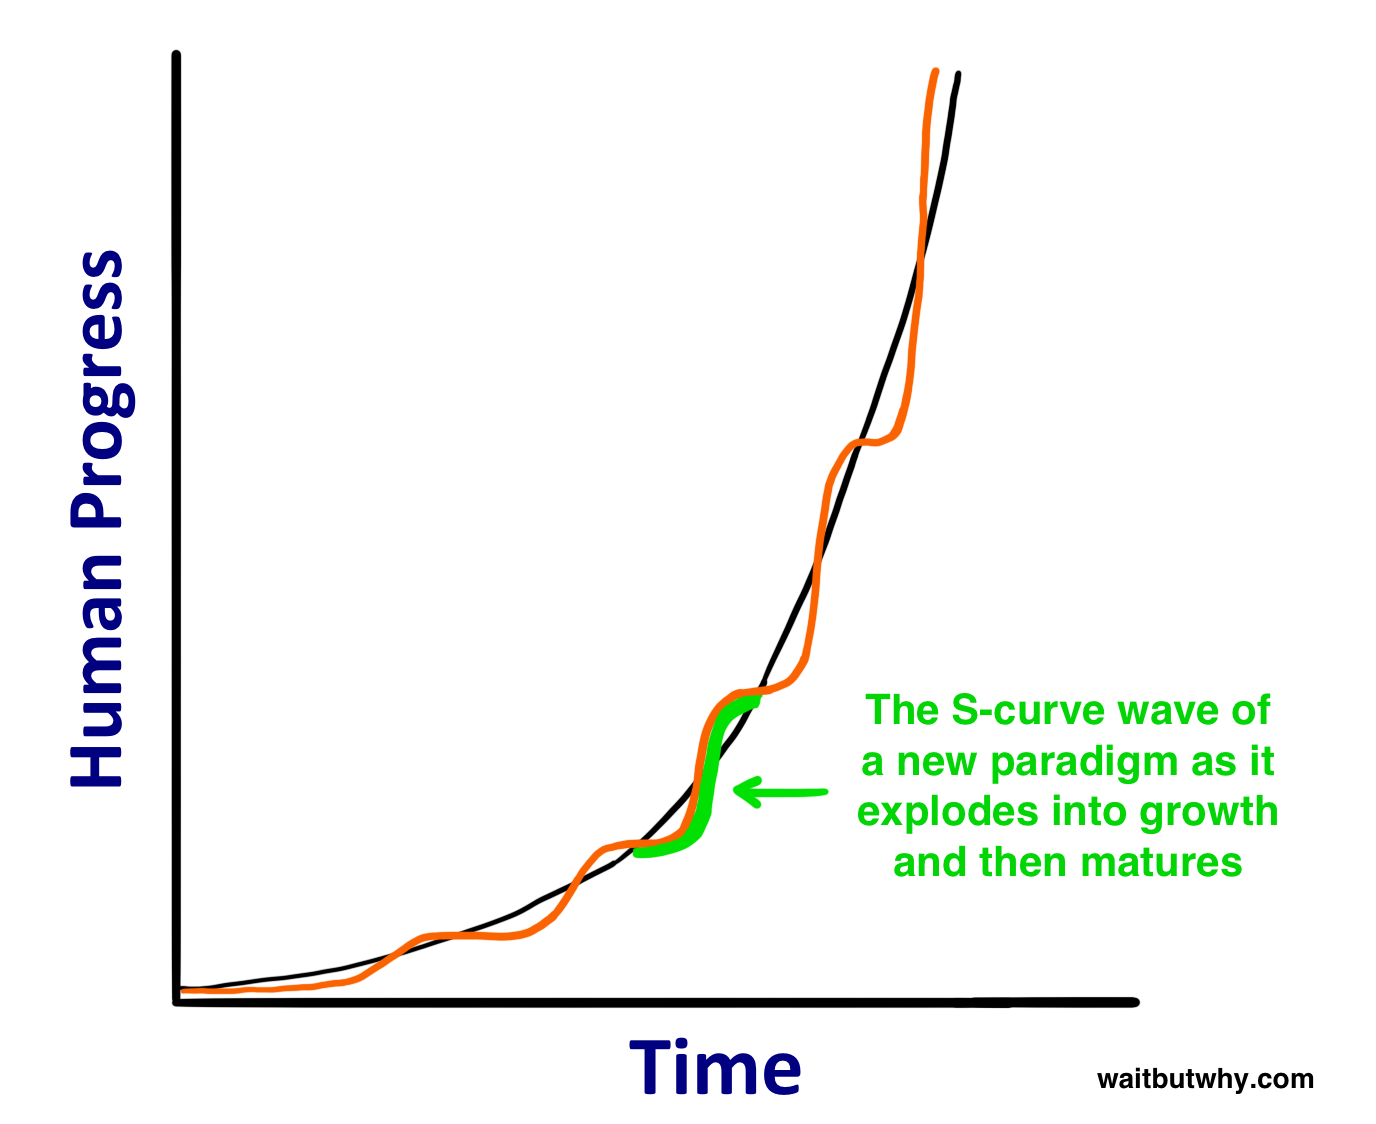
\includegraphics[width=0.48\textwidth]{curvyexponential.png}
  \end{center}
  \caption{Inexorable Progress}
\end{wrapfigure}

Even without Moore's Law, there is one fact that many quote as the driving reason why we must reach AGI (and, soon after, ASI): human progress is, historically, exponential\cite{wbw}. It may seem to slow for periods at a time, but eventually we make such leaps and bounds that society quickly becomes unrecognizable. Society is vastly different in 2015 from that of 1800, due to the progress we've made in the past 200 years. But we would have much further back, much more than 200 years, from 1800, in order to reach the same level of change.

However, despite our newfound assurance that progress \textit{will} happen, we still seem to be incapable of predicting what form it will take. It has been decades since we were first convinced that flying cars were to be the way of the future, and as of 2015 we still drive ours along the same old paved roads.

Hence my argument becomes not that the human race \textit{won't} progress, but rather that we simply don't know what that innovation will look like. For certain we cannot know that ASI is the form our next big leap will take.

%----------------------------------------------------------------------------------------
%	Conclusion
%----------------------------------------------------------------------------------------

\section{Conclusion} % Major section

I will not say that AGI and ASI are impossible parts of our (very near) future. Rather, I wish to emphasize that, with exponential growth meaning quicker and quicker change, we are in a time where we are suddenly unable to predict even a decade into the future; those ten years may result in more change than the entire past century. However, it is also possible that 2025 may come and go without much change from our current situation.

I will not, however, believe claims stating that AGI is imminent purely based on the inexorable march of Moore's Law. While Moore's Law is projected to hold out for at least another decade, even today its progress is slowing and it cannot be relied upon as the driving force behind producing \textit{true} artificial intelligence. What I will believe is, within my lifetime, we will see many more changes that dramatically alter society, quite likely more drastically than in the past \textit{millennium}. But we have no way of knowing what form those changes will take, or even if they will be instigated by technology as we currently understand it.

Artificial Narrow Intelligence is a powerful force in our world today. Artificial General Intelligence has the power to easily change our world. Artificial Super Intelligence has the power to easily \textit{end} our world. But none of it is guaranteed to happen, at least not as the experts seem convinced is imminent.

%----------------------------------------------------------------------------------------
%	BIBLIOGRAPHY
%----------------------------------------------------------------------------------------

\newpage % Begins the references on a new page instead of on the same page as the essay 

\bibliographystyle{plain}
\bibliography{the-singularity}

%----------------------------------------------------------------------------------------

\end{document}